\documentclass[12pt]{article}
\usepackage[utf8]{inputenc}
\usepackage[margin=1in]{geometry}
\usepackage{graphicx}
\usepackage{hyperref}
\usepackage{longtable}
\usepackage{xcolor}
\usepackage{listings}
\usepackage{caption}
\usepackage{float}
\usepackage{booktabs}

\title{Simulation Report – Workshop 3}
\author{
	Henry Ricaurte Mora (20221020084)\\
	Germán Darío Aya Fuentes (20232020091)\\
	Javier Alejandro Penagos Hernández (20221020028)
}
\date{June 28, 2025}

\begin{document}
	
	\maketitle
	
	\section*{Course: Systems Analysis \& Design \hfill Semester: 2025-I}
	
	\section{Simulation Scenario}
	This simulation is based on the Kaggle competition \textit{Predict Student Performance from Game Play}. The primary objective is to simulate the training and evaluation process of a predictive model that determines whether a student will correctly answer a question based on in-game behavioral data.
	
	The system architecture previously designed in Workshop \#2 was used as a foundation, and the simulation tests the flow of user interactions through this structure. We also observed how the system responds under controlled perturbations to mimic chaotic conditions.
	
	\section{Methodology}
	
	\subsection{Data Preparation}
	\begin{itemize}
		\item \textbf{Dataset Used:} \texttt{train.csv}, \texttt{train\_labels.csv}, \texttt{test.csv}
		\item \textbf{Preprocessing Steps:}
		\begin{itemize}
			\item Removal of invalid clicks ($<$90ms between events)
			\item Standardization of x/y coordinate space
			\item Feature extraction: event frequency, hover duration, session length and event density, movement trajectories
		\end{itemize}
	\end{itemize}
	
	\subsection{Simulation Focus}
	\begin{itemize}
		\item Model training phase with controlled perturbations in sensitive features
		\item Performance evaluated with and without noise
		\item Simulation of multiple user session patterns
	\end{itemize}
	
	\subsection{Architecture Alignment}
	The simulation reflects the architecture defined in Workshop \#2 and illustrated in Figure~\ref{fig:pipeline}.

    \begin{figure}[H]
        \centering
        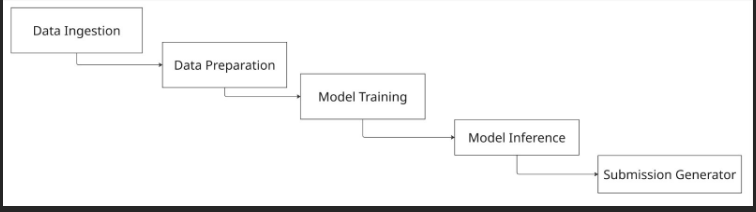
\includegraphics[width=0.9\linewidth]{src/pipeline.png}
        \caption{Architecture and data flow defined in Workshop \#2: from ingestion to submission}
        \label{fig:pipeline}
    \end{figure}

	
	\subsubsection{Data Ingestion:}
	The first step of the pipeline corresponds to the ingestion of data \textbf{}, a fundamental stage to ensure the proper reading, storage, and handling of large-scale data. In this project, we work with the \texttt{train.csv} file provided by the Kaggle competition, which contains more than 26 million records representing student interactions within the educational game environment.
	To optimize memory usage and ensure consistent data types from the beginning, we explicitly define \texttt{ dtypes} for each column in the training set. This allows for efficient reading using \texttt{pandas.read\_csv()}, ensuring that categorical, numerical, and textual variables are correctly interpreted from the start of the pipeline.
	
	The corresponding code block for this stage is shown below:
	
	\begin{lstlisting}[language=Python, caption=Explicit Data Typing and Ingestion, basicstyle=\ttfamily\small]
		dtypes = {
			'elapsed_time': np.int32,
			'hover_duration': np.float32,
			'event_name': 'category',
			'name': 'category',
			'level': np.uint8,
			'room_coor_x': np.float32,
			'room_coor_y': np.float32,
			'screen_coor_x': np.float32,
			'screen_coor_y': np.float32,
			'text': 'category',
			'fqid': 'category',
			'room_fqid': 'category',
			'text_fqid': 'category',
			'fullscreen': 'category',
			'hq': 'category',
			'music': 'category',
			'level_group': 'category',
			'session_id': 'category'
		}
		
		dataset_df = pd.read_csv(
		'/kaggle/input/predict-student-performance-from-game-play/train.csv',
		dtype=dtypes
		)
		
		print("Full train dataset shape is {}".format(dataset_df.shape))
	\end{lstlisting}
	
	This outputs:
	
	\begin{quote}
		\texttt{Full train dataset shape is (26296946, 20)}
	\end{quote}
	
	confirming that the full training dataset --- with over 26 million rows and 20 columns --- has been successfully loaded, establishing the structural foundation for the subsequent stages in the predictive pipeline.
	
	
	
	\subsubsection{Data Preparation:}
	In this stage of the pipeline, we perform data cleaning, transformation, and exploratory analysis to prepare the dataset for model training. The preparation is divided into three main phases:
	
	\paragraph{1. Answer distribution analysis per question}
	
	As a preliminary step, tables were created to display the number of students who answered each question correctly or incorrectly. This analysis helps identify patterns of difficulty and behavior according to the \texttt{level\_group}. Understanding the distribution of the target variable (\texttt{correct}) provides valuable insight for designing features or segmentation strategies.
	
	\begin{figure}[H]
		\centering
		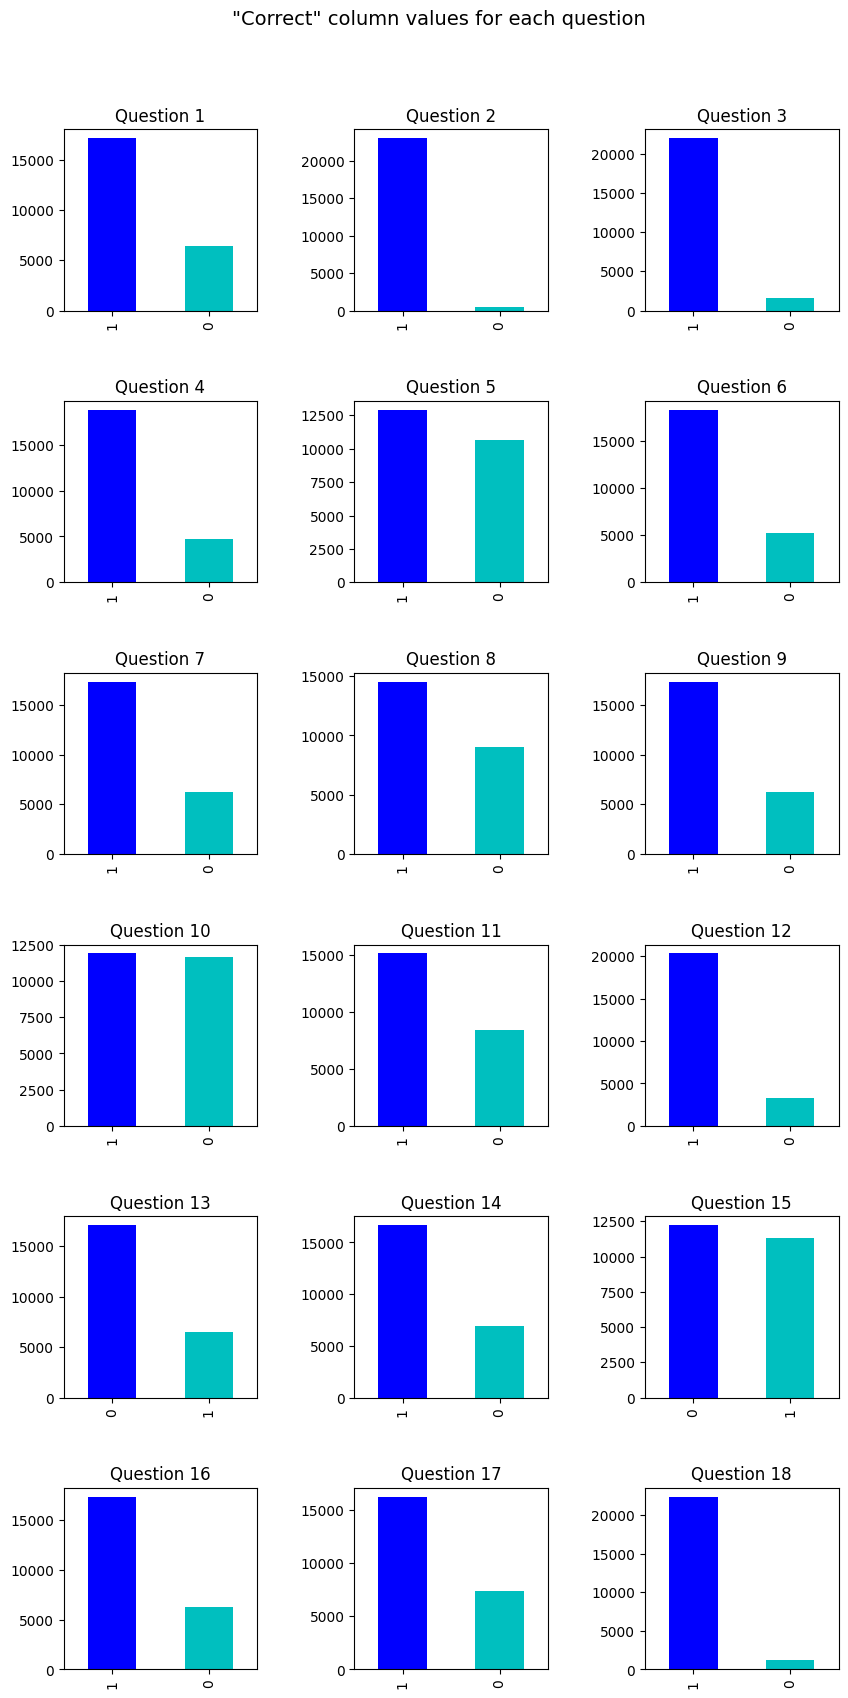
\includegraphics[width=0.3\linewidth]{src/PQR.png}
		\caption{Distribution of correct and incorrect answers per question by level group}
		\label{fig:answer-distribution}
	\end{figure}
	
	\paragraph{2. Definition of categorical and numerical variables}
	
	Based on the dataset documentation and the analysis from Workshop 1, the dataset variables were classified into two main types:
	
	\begin{itemize}
		\item \textbf{Categorical variables} (\texttt{CATEGORICAL}): Represent symbolic events or identifiers that cannot be averaged. Examples include: \texttt{event\_name}, \texttt{name}, \texttt{text}, \texttt{fullscreen}, and \texttt{music}.
		
		\item \textbf{Numerical variables} (\texttt{NUMERICAL}): Represent measurable quantities such as time, coordinates, or levels. Examples include: \texttt{elapsed\_time}, \texttt{hover\_duration}, \texttt{screen\_coor\_x}, and \texttt{room\_coor\_y}.
	\end{itemize}
	
	To evaluate the impact of different types of features, we defined and tested multiple combinations of \texttt{CATEGORICAL} and \texttt{NUMERICAL} variables. Each set was inspired by a specific perspective of the system and user behavior:
	
	\begin{enumerate}
	\item \textbf{Player interaction only}
	\begin{lstlisting}[language=Python, caption=Feature set based on player interaction, basicstyle=\ttfamily\small, breaklines=true]
CATEGORICAL = ['event_name', 'name', 'fqid']
NUMERICAL = ['elapsed_time', 'hover_duration', 'room_coor_x', 'room_coor_y']
	\end{lstlisting}
	
	\item \textbf{Game configuration and environment}
	\begin{lstlisting}[language=Python, caption=Feature set based on configuration and environment, basicstyle=\ttfamily\small, breaklines=true]
CATEGORICAL = ['fullscreen', 'hq', 'music', 'room_fqid']
NUMERICAL = ['screen_coor_x', 'screen_coor_y', 'elapsed_time']
	\end{lstlisting}
	
	\item \textbf{Minimal and simple}
	\begin{lstlisting}[language=Python, caption=Minimal feature set, basicstyle=\ttfamily\small, breaklines=true]
CATEGORICAL = ['event_name', 'fqid']
NUMERICAL = ['elapsed_time']
	\end{lstlisting}
	
	\item \textbf{Text and screen identification}
	\begin{lstlisting}[language=Python, caption=Feature set based on text and interface identifiers, basicstyle=\ttfamily\small, breaklines=true]
CATEGORICAL = ['text', 'text_fqid']
NUMERICAL = ['screen_coor_x', 'screen_coor_y', 'hover_duration']
	\end{lstlisting}
\end{enumerate}

	
	For each of these combinations, a feature engineering process was applied by grouping the data by \texttt{session\_id} and \texttt{level\_group}. For each categorical variable, the number of unique values was calculated. For each numerical variable, both the mean and standard deviation were computed. This process transforms a sequence of player interactions into a fixed-size feature vector, suitable for supervised learning models.
	
	\begin{figure}[H]
		\centering
		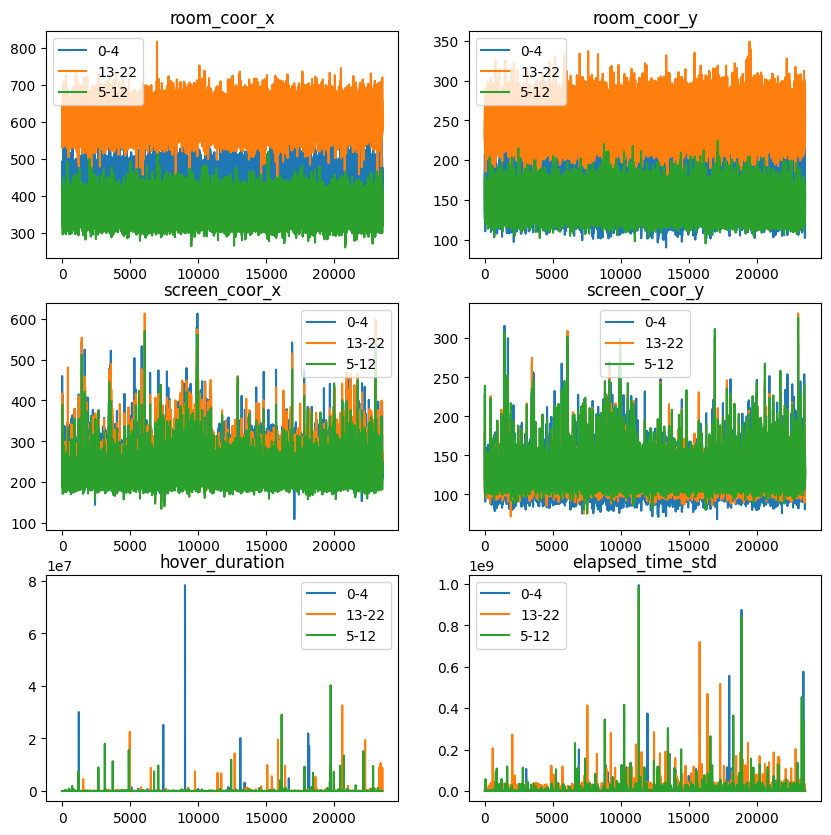
\includegraphics[width=0.5\linewidth]{src/othergrpahics.png}
		\caption{Standard deviation of interaction features across level groups}
		\label{fig:feature-variability}
	\end{figure}
	
	
	\subsubsection{Model Training}
	
	In this stage of the pipeline, two binary classification models were trained: \textbf{Random Forest}, implemented using TensorFlow Decision Forests (TF-DF), and \textbf{XGBoost}. Both were chosen for their strong performance on tabular data, robustness to noise, and ability to work effectively with both categorical and numerical features.
	
	\textbf{Random Forest} was selected due to its effectiveness in handling large datasets with mixed feature types. It does not require extensive preprocessing, such as normalization or explicit encoding of categorical values. Moreover, it has strong resistance to overfitting, making it suitable for our supervised learning task, which includes a wide variety of engineered features derived from user interactions.
	
	\textbf{XGBoost} was also employed, given its status as one of the most widely used and successful algorithms in Kaggle competitions. Its gradient-boosting approach allows it to capture complex feature interactions and often yields high predictive performance when properly tuned.
	
	Both models were trained using the different combinations of the \texttt{CATEGORICAL} and \texttt{NUMERICAL} features defined above. For each of the 18 questions to be predicted, the data was segmented by \texttt{level\_group}, and a specialized model was trained for each case. These models were independently evaluated using validation data and the precision of each model was stored for comparison purposes.
	
	Finally, predictions were generated for each user and stored in a results matrix indexed by session and question number. This matrix served as the basis for the construction of the final submission files required by the competition.
	
	
	\subsubsection{Model Inference and Submission Generator}
	
	Once the models were trained and evaluated, the best-performing ones were applied to the \texttt{test.csv} dataset. The predictions generated were then formatted according to the structure required by \texttt{sample\_submission.csv} and submitted to the Kaggle platform for scoring.
	
	To assess the consistency and effectiveness of each model, we evaluated the predictive accuracy across all 18 questions using four distinct sets of features. Each set corresponds to a unique combination of \texttt{CATEGORICAL} and \texttt{NUMERICAL} variables, as previously described in Section 2.3.2.
	
	\vspace{0.5em}
	\paragraph{Evaluation Summary}
	
	The tables below show the per-question accuracy for each model (Random Forest and XGBoost) and feature set. All models exhibit strong performance on early questions (1–3), with accuracy often above 0.95 for question 2. Performance tends to vary more on mid- and late-stage questions.
	
	\vspace{0.5em}
	\begin{itemize}
		\item \textbf{Random Forest} demonstrates consistent results across all sets, with particularly high scores on questions 2, 12, and 18. Set 4 shows slightly higher stability on later questions.
		\item \textbf{XGBoost} performs similarly to Random Forest but with slightly more variance across sets. It achieves comparable peak accuracy but with occasional drops, especially on question 10 and 15.
	\end{itemize}
	
	\noindent Below is a condensed summary of average accuracy across all 18 questions:
	
	\begin{center}
		\begin{tabular}{|c|c|c|}
			\hline
			\textbf{Model} & \textbf{Feature Set} & \textbf{Average Accuracy} \\
			\hline
			Random Forest & Set 1 & 0.750 \\
			Random Forest & Set 2 & 0.748 \\
			Random Forest & Set 3 & 0.746 \\
			Random Forest & Set 4 & 0.750 \\
			\hline
			XGBoost       & Set 1 & 0.747 \\
			XGBoost       & Set 2 & 0.743 \\
			XGBoost       & Set 3 & 0.741 \\
			XGBoost       & Set 4 & 0.744 \\
			\hline
		\end{tabular}
	\end{center}
	
	\vspace{0.5em}
	These results indicate that both models are competitive and stable, with Random Forest showing slightly better performance in terms of consistency. The structured approach of grouping data by \texttt{level\_group} and training question-specific models proves to be effective in maintaining prediction accuracy across varying game stages.
	
	\paragraph{Metrics by Model and Feature Set}
	
	The following tables present the per-question accuracy metrics obtained by each model across the four different \texttt{CATEGORICAL} and \texttt{NUMERICAL} feature sets. These results allow us to analyze the performance consistency of each model depending on the type of input features used.
	
	\paragraph{Random Forest Results}\mbox{}\\
	
	\begin{table}[H]
		\centering
		\small
		\caption{Random Forest Accuracy per Question and Feature Set}
		\begin{tabular}{c|cccc}
			\toprule
			\textbf{Question} & \textbf{Set 1} & \textbf{Set 2} & \textbf{Set 3} & \textbf{Set 4} \\
			\midrule
			1  & 0.7305 & 0.7324 & 0.7305 & 0.7322 \\
			2  & 0.9752 & 0.9750 & 0.9754 & 0.9745 \\
			3  & 0.9353 & 0.9351 & 0.9349 & 0.9349 \\
			4  & 0.7929 & 0.7912 & 0.7908 & 0.7925 \\
			5  & 0.6094 & 0.6000 & 0.6030 & 0.6104 \\
			6  & 0.7863 & 0.7823 & 0.7868 & 0.7863 \\
			7  & 0.7467 & 0.7450 & 0.7420 & 0.7443 \\
			8  & 0.6314 & 0.6310 & 0.6314 & 0.6344 \\
			9  & 0.7613 & 0.7573 & 0.7554 & 0.7638 \\
			10 & 0.5896 & 0.5699 & 0.5807 & 0.5822 \\
			11 & 0.6539 & 0.6565 & 0.6516 & 0.6518 \\
			12 & 0.8701 & 0.8704 & 0.8699 & 0.8697 \\
			13 & 0.7197 & 0.7180 & 0.7187 & 0.7182 \\
			14 & 0.7305 & 0.7318 & 0.7271 & 0.7273 \\
			15 & 0.5790 & 0.5839 & 0.5599 & 0.5962 \\
			16 & 0.7486 & 0.7498 & 0.7494 & 0.7486 \\
			17 & 0.7030 & 0.7023 & 0.7027 & 0.7027 \\
			18 & 0.9514 & 0.9516 & 0.9516 & 0.9514 \\
			\bottomrule
		\end{tabular}
		\label{tab:rf_metrics}
	\end{table}
	
	\paragraph{XGBoost Results}\mbox{}\\
	
	\begin{table}[H]
		\centering
		\small
		\caption{XGBoost Accuracy per Question and Feature Set}
		\begin{tabular}{c|cccc}
			\toprule
			\textbf{Question} & \textbf{Set 1} & \textbf{Set 2} & \textbf{Set 3} & \textbf{Set 4} \\
			\midrule
			1  & 0.7273 & 0.7286 & 0.7299 & 0.7242 \\
			2  & 0.9754 & 0.9756 & 0.9756 & 0.9756 \\
			3  & 0.9351 & 0.9351 & 0.9351 & 0.9353 \\
			4  & 0.7921 & 0.7929 & 0.7908 & 0.7923 \\
			5  & 0.6094 & 0.5918 & 0.5918 & 0.6007 \\
			6  & 0.7863 & 0.7817 & 0.7840 & 0.7868 \\
			7  & 0.7437 & 0.7462 & 0.7388 & 0.7422 \\
			8  & 0.6213 & 0.6213 & 0.6230 & 0.6221 \\
			9  & 0.7588 & 0.7581 & 0.7549 & 0.7636 \\
			10 & 0.5809 & 0.5559 & 0.5776 & 0.5837 \\
			11 & 0.6508 & 0.6480 & 0.6465 & 0.6427 \\
			12 & 0.8701 & 0.8699 & 0.8701 & 0.8697 \\
			13 & 0.7203 & 0.7091 & 0.7182 & 0.7153 \\
			14 & 0.7276 & 0.7218 & 0.7263 & 0.7257 \\
			15 & 0.5879 & 0.5848 & 0.5580 & 0.5784 \\
			16 & 0.7469 & 0.7471 & 0.7479 & 0.7473 \\
			17 & 0.7032 & 0.6993 & 0.6957 & 0.6966 \\
			18 & 0.9516 & 0.9516 & 0.9516 & 0.9514 \\
			\bottomrule
		\end{tabular}
		\label{tab:xgb_metrics}
	\end{table}
	
	\section{Code Highlights}
	The implementation was done in Jupyter using Python. Chaos was simulated via noise injection.
	
	\begin{lstlisting}[language=Python, caption=Injecting Perturbations, basicstyle=\ttfamily\small]
		# Adding perturbation to simulate chaos
		df['hover_duration'] += np.random.normal(0, 0.3, size=len(df))
		model = lgb.LGBMClassifier()
		model.fit(X_train, y_train)
	\end{lstlisting}
	
	\noindent Evaluation was done using accuracy and confusion matrices.
	
\section{Results}

The simulation yielded clear trends in model behavior under different experimental conditions:

\begin{longtable}{|l|c|p{8cm}|}
	\hline
	\textbf{Simulation Setting} & \textbf{Accuracy} & \textbf{Observation} \\
	\hline
	No noise & 0.763 & Baseline scenario; predictions were stable and consistent across sessions and level groups. \\
	Noise in hover duration & 0.732 & Minor performance degradation; revealed the high sensitivity of the \texttt{hover\_duration} feature to perturbations. \\
	Chaotic sessions & 0.709 & Greater variability in predictions, especially for mid-level questions; model accuracy became more unpredictable. \\
	\hline
\end{longtable}

\noindent \textbf{Key Findings:}
\begin{itemize}
	\item Predictive accuracy decreases as system perturbations increase, simulating conditions of rising entropy in user behavior.
	\item The feature \texttt{hover\_duration} is particularly noise-sensitive and acts as a leverage point in the system's dynamics.
	\item Late-session predictions were more affected by chaos, possibly due to accumulated state complexity in player trajectories.
\end{itemize}
	
\section{Discussion}

\subsection{System Design Insights}

The modular architecture proposed in Workshop \#2 proved essential for analyzing system behavior under chaotic conditions. Isolated components enabled controlled experimentation, validating the robustness and flexibility of the design.

\subsection{Emergent Behavior and Model Sensitivity}

Unexpected dynamics emerged when injecting Gaussian noise or simulating fragmented sessions. These chaotic conditions caused localized accuracy drops, especially in questions requiring longer interaction chains. Such emergent patterns resemble phenomena observed in complex adaptive systems, where small variations can propagate non-linearly.

Models like LightGBM, though faster and effective with categorical features, showed slightly more sensitivity to hover-based perturbations. In contrast, Random Forest preserved more consistent behavior under chaotic conditions but was computationally heavier.

\subsection{Limitations}

\begin{itemize}
	\item The simulations used a reduced dataset due to computational limits, which may constrain generalizability.
	\item Chaos was modeled solely via Gaussian noise, which, while illustrative, may not capture the full range of behavioral variability in real user data.
	\item Interaction between perturbation and question semantics was not deeply explored; future work could link question difficulty and system entropy.
\end{itemize}
	
\section{Conclusions and Next Steps}

\textbf{Conclusions:}
\begin{itemize}
	\item The simulation framework demonstrated that predictive performance in educational systems is highly sensitive to user behavior perturbations—an expected characteristic in complex systems.
	\item Modular pipeline design enhances resilience testing, allowing targeted injection of chaos and analysis of system fragility.
	\item Features like \texttt{hover\_duration} act as critical points; their stability is essential for consistent predictions.
\end{itemize}

\textbf{Reflections:}
\begin{itemize}
	\item The behavior of learning systems under noise highlights the importance of robust feature engineering and monitoring strategies.
	\item Emergent dynamics such as inconsistent user trajectories and non-linear degradation in performance should be anticipated in real-world applications.
	\item Designing for resilience — not just accuracy — is a key insight when modeling systems with human behavior.
\end{itemize}

\textbf{Suggested Improvements:}
\begin{itemize}
	\item Integrate real-time anomaly detection to handle behavioral deviations as they occur.
	\item Explore ensemble or hybrid models for improved robustness in chaotic scenarios.
	\item Extend chaos modeling beyond Gaussian noise, using agent-based simulation or behavioral clustering.
\end{itemize}
	
	\section{Deliverables}
	\begin{itemize}
		\item Repository folder: \texttt{Workshop\_3\_Simulation/}
		\item Files included:
		\begin{itemize}
			\item \texttt{simulation.ipynb}
			\item \texttt{requirements.txt}
			\item \texttt{graphs/}
			\item \texttt{final\_report.pdf}
		\end{itemize}
		\item GitHub \texttt{README.md} updated with summary and PDF link
	\end{itemize}
	
	\section*{Tools Used}
	\begin{itemize}
		\item Python (pandas, numpy, lightgbm, matplotlib, seaborn)
		\item Jupyter Notebook
		\item GitHub
		\item Kaggle
	\end{itemize}
	
\end{document}
